\section{An Algorithm for Relaxed Ring Loading}
\label{sec:relaxed-ring-loading}

In this section, we derive the exact, polynomial-time algorithm for \RRL invented by \citet{schrijver99}.
Considering that we want to use the real-valued routing obtained from this algorithm to approximate an optimal binary routing, it is desirable to determine such a real-valued routing $\Phi$ in which all but at most $\lfloor \frac{n}{2} \rfloor$ demands are already routed all front or all back.

\subsection{Minimal Solutions}

Minimal solutions have this property:

\begin{definition}
	Let $\Phi^\ast$ be an optimal solution to an instance of \RRL.
	We say that $\Phi^\ast$ is \emph{minimal} if there exists no other optimal routing $\Phi'$ such that $L_i(\Phi') \leq L_i(\Phi^\ast)$ for all $1 \leq i \leq n$ and $L_j(\Phi') < L_j(\Phi^\ast)$ for at least one $j$.
\end{definition}
While this definition might seem arbitrary at first glance, minimal solutions are of a particularly aesthetic form.

\begin{theorem}
	\label{theo:number-of-splits}
	Let $\Phi^\ast$ be a minimal solution to an instance of \RRL of size $n$.
	Then $\Phi^\ast$ splits at most $\lfloor \frac{n}{2} \rfloor$ demands.
\end{theorem}

This result is quite remarkable, as we can have up to $\binom{n}{2} = \frac{n(n-1)}{2}$ non-zero demands.
Before proving the theorem, it is sensible to introduce some additional notation and terminology.
From now on, we consider the \RRL instance $I$ of size $n \in \N$ as fixed.
\begin{notation}
	Let $i, j \in \N$ with $i < j$.
	We define the half-open interval $[i, j) \coloneqq \{i, i+1, \ldots, j-1\}$.
\end{notation}

\begin{definition}
	Let $i, j, u, v \in [n]$, $i < j, u < v$ and $d_{i,j}, d_{u, v}$ be two demands of a \RRL instance.
	We say that
	\begin{enumerate}
		\item $d_{i, j}$ and $d_{u, v}$ are \emph{crossing} if $i, j, u, v$ are pairwise distinct and $i < u < j < h$ or $u < i < h < j$.
		\item $d_{i, j}$ and $d_{u, v}$ are \emph{parallel} if they are not crossing.
		\item If $d_{i, j}$ and $d_{u, v}$ are parallel, the edge $\{k, k+1\}$ is \emph{in between}
		$d_{i,j}$ and $d_{u, v}$ if it lies on the front route of exactly one of the demands.
		\Todo{fix definition.}
	\end{enumerate}
\end{definition}
Crossing and parallel demands are most easily understood visually.
See \cref{fig:parallel-demands} for some examples.

\begin{figure}
	\centering
	\begin{subfigure}[t]{.4\textwidth}
		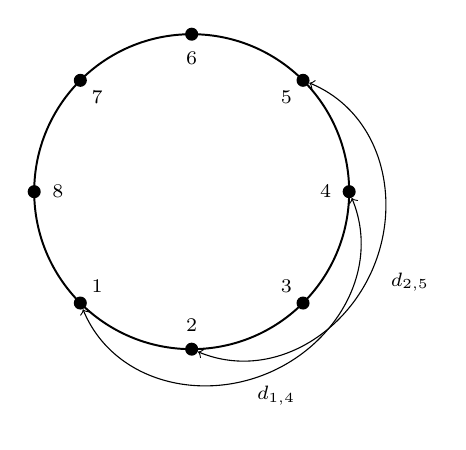
\begin{tikzpicture}[font=\scriptsize, node/.style={circle,thick,draw},
		l_2/.style={line width =0.25mm},
		scale=1, transform shape]
		% equidistant points and arc
		\foreach \x [count=\p] in {0,...,7} {
			\node[shape=circle,fill=black, scale=0.5] (\p) at (\x*45-135:2) {};
		};
		\foreach \x [count=\p] in {0,...,7} {
			\draw (225 + \x*45:1.7) node {\p};
			%				\draw (-30-\x*60:2.4) node {$\bar{\p}$};
		}; 
		\draw[l_2] (4) arc (0:360:2);
		\node (a) at (-22.5:3) {$d_{2, 5}$};
		\draw[<->] (2)  to [out=-22.5,in=-112.5] (-22.5:2.5) to [out=67.5,in=-22.5](5);
		\node (b) at (-67.5:2.8) {$d_{1, 4}$};
		\draw[<->] (1)  to [out=-67.5,in=-157.5] (-67.5:2.5) to [out=22.5,in=-67.5] (4);
		
		\node (bottom) at (0, -2.8) {};
		%		\draw[dashed] (1) -- (3) -- (5) -- (1);
		% axes
		%		\draw [dotted, gray] (-2.6,0) -- (2.6,0);
		%		\draw [dotted, gray] (0,-2.15) -- (0,2.15);
		\end{tikzpicture}
		\subcaption{$d_{1, 4}$ and $d_{2, 5}$ are crossing.}
	\end{subfigure}
%	\hspace{1cm}
	\begin{subfigure}[t]{.4\textwidth}
		\captionsetup{width=1.1\linewidth}
		\begin{tikzpicture}[font=\scriptsize, node/.style={circle,thick,draw},
		l1_green/.style={thick, green!80!black},
		l1_red/.style={thick, blue!80!white},
		l_2/.style={},
		l_3/.style={line width =0.25mm},
		scale=1, transform shape]
		\draw[l_3] (2, 0) arc (0:360:2);
		
		\draw[l1_green] (5) arc (45:90:2);
		\draw[l1_green] (8) arc (180:270:2);
		\draw[l1_red] (4) arc (0:45:2);
		% equidistant points
		\foreach \x [count=\p] in {0,...,7} {
			\node[shape=circle,fill=black, scale=0.5] (\p) at (\x*45-135:2) {};
		};
		% labels
		\foreach \x [count=\p] in {0,...,7} {
			\draw (225 + \x*45:1.7) node {\p};
			%				\draw (-30-\x*60:2.4) node {$\bar{\p}$};
		};
		
		\node (a) at (10:2.9) {$d_{2, 5}$};
		\draw[l_2, <->] (2)  to [out=-22.5,in=-112.5] (-22.5:2.8) to [out=67.5,in=-22.5](5);
		
		\node (b) at (-15:2.46) {$d_{2, 4}$};
		\draw[l_2,<->] (2)  to [out=-15,in=-135] (-45:2.25) to [out=45,in=-75] (4);
		
		\node (c) at (135:2.7) {$d_{6, 8}$};
		\draw[l_2, <->] (6)  to [out=157.5,in=45] (135:2.4) to [out=-135,in=112.5] (8);
		
		\node (bottom) at (0, -2.8) {};
		%		\draw[dashed] (1) -- (3) -- (5) -- (1);
		% axes
		%		\draw [dotted, gray] (-2.6,0) -- (2.6,0);
		%		\draw [dotted, gray] (0,-2.15) -- (0,2.15);
		\end{tikzpicture}
		\subcaption{$d_{2,4}$, $d_{2, 5}$ and $d_{6, 8}$ are pairwise parallel.}
	\end{subfigure}
	\caption{Examples of crossing and parallel demands.
		In (b), the green edges lie in between $d_{2, 5}$ and $d_{6, 8}$.
		The blue edge is the only edge in between $d_{2, 4}$ and $d_{2, 5}$.}
	\label{fig:parallel-demands}
\end{figure}
Next, we prove the following lemma.

\begin{lemma}
	\label{lemma:parallel-demands}
	Let $\Phi^\ast$ be a minimal routing and $d_{i, j}$ and $d_{u, v}$ be parallel demands.
	Then no edge in between $d_{i, j}$ and $d_{u, v}$ carries traffic from both demands.
\end{lemma}
\begin{proof}
	Let $\Phi^\ast$ be a minimal solution and assume that the edge $\{k, k+1\}$ lies in between two parallel demands $d_{i, j}, d_{u, v}$ and carries traffic from both demands.
	Let $\alpha$ and $\beta$ be the amounts of traffic from $d_{i,j}$ and $d_{u, v}$, respectively, that are routed through $\{k, k+1\}$.
	Furthermore, assume w.l.o.g. that $\alpha \leq \beta$ and that $\{k, k+1\}$ lies on the front route of $d_{i, j}$ (the other cases can be reasoned analogously).
	
	We now construct a new routing $\Phi'$ from $\Phi^\ast$ by rerouting traffic $\alpha$ of both demands such that it no longer passes through $\{k, k+1\}$.
	This results in $d_{i, j}$ being routed all front or all back.
	The rerouting of $d_{i, j}$ causes the loads on all edges on its front route to decrease by $\alpha$ and those on the back route to increase by $\alpha$.
	Similarly, the rerouting of $d_{u, v}$ increases the loads on all edges on its back route by $\alpha$ and decreases those on its front route by $\alpha$.
	
	Let $\{l, l+1\}$ be any edge.
	Then we can write the load under the new routing as
	\begin{equation}
	L_l(\Phi') = L_l(\Phi^\ast) 
	+ \alpha (\dOne_{\{l \notin [i, j)\}} - \dOne_{\{l \in [i, j)\}} +  \dOne_{\{l \in [g, h)\}} - \dOne_{\{l \notin [g, h)\}} )
	\end{equation}
	Here, $\dOne_{\{\ldots\}}$ is the indicator function that is $1$ if the condition in the index is true and $0$ else.
	We assumed that $\{k, k+1\}$ lies on the front route of $d_{i, j}$, but also that it lies in between $d_{i, j}$ and $d_{g, h}$.
	This implies that $[g, h] \subset [i, j]$.
	Hence $l \notin [i, j)$ and $l \in [g, h)$ cannot both be true at the same time.
	This shows that $L_l(\Phi') \leq L_l(\Phi^\ast)$.
	Furthermore, $k \in [i, j)$ and $k \notin [g, h)$ by definition of $k$.
	Thus we have $L_k(\Phi') < L_k(\Phi^\ast)$.
	Altogether, the existence of the routing $\Phi'$ contradicts the minimality of $\Phi^\ast$.
\end{proof}

With these preparations, we can now conduct the proof of \cref{theo:number-of-splits}.
\begin{proof}[Proof of \cref{theo:number-of-splits}]
	Let $\Phi^\ast$ be a minimal routing and let $S \coloneqq \{(i, j)\ |\ 0 < \Phi^\ast(i, j) < 1\}$ be the set of indices of demands that are split by $\Phi^\ast$.
	Furthermore, let $(i, j), (u, v) \in S$.
	
	If the demands $d_{i,j}$ and $d_{u, v}$ were parallel, there would be a link $\{k, k+1\}$ that carries traffic from both demands, as they are both split.
	However, it follows from the minimality of $\Phi^\ast$ and \cref{lemma:parallel-demands} that this cannot be the case, which implies that $d_{i,j}$ and $d_{u, v}$ are crossing.
	This requires, by definition, that $i, j, u, v$ are mutually distinct.
	
	This implies that every element of $[n]$ can occur in at most one tuple in $S$.
	As the tuples in $S$ each consist of two elements, there can be at most $\lfloor\frac{n}{2}\rfloor$ such tuples.
\end{proof}

The existence of minimal solutions is not clear, a priori.
In the following, we will show that minimal solutions always exist by providing an algorithm.

\subsection{\RRL with Capacities}

In order to construct a minimal solution, we first consider a generalization of \RRL by appending an edge capacity $C_k \in \R_{\geq 0}$ for each edge $\{k, k+1\}$.
The resulting problem, \textsc{RelaxedRingLoadingWithCapacities} (\RRLWC), is to determine a real-valued routing $\Phi^\ast$ such that $L_k(\Phi^\ast) \leq C_k$ for all $k \in [n]$.
We denote instance of this problem with $(I, C)$, where $I$ is an \RRL instance and $C = (C_k)_{k \in [n]}$ the capacities.
This problem does not always have feasible solutions.
In the following, we show a necessary and sufficient condition for the existence of feasible solutions.

\begin{definition}
	A \emph{cut} $\{g, h\}$ is a set of two distinct edges $\{g, g+1\}$, $\{h, h+1\}$.
\end{definition}

We can imagine a cut $\{g, h\}$ as a chord connecting the midpoints of the edges $\{g, g+1\}$ and $\{h, h+1\}$.
A cut therefore "splits" the ring into two parts.

\begin{definition}
	Let $d_{i, j}$ be a demand and $\{g, h\}$ a cut with $g < h$.
	\begin{enumerate}
		\item We say that $d_{i, j}$ \emph{crosses} $\{g, h\}$ if the endpoints of $d_{i, j}$ are on both sides of the cut.
		Formally, this is the case if and only if $\abs{\{i, j\} \cap (g, h]} = 1$.
		\item $d_{i, j}$ is \emph{parallel} to $\{g, h\}$ if it does not cross $\{g, h\}$.
		\item Two cuts are \emph{crossing} or \emph{parallel} in the same sense two demands are.
		\item The \emph{demand across the cut} $\{g, h\}$ is the sum of demands with endpoints on both sides of the cut:
		\begin{equation}
			\label{eq:cut-demand-definition}
			D_{g,h} \coloneqq \sum_{d_{i,j} \text{ crosses } \{g, h\} } d_{i, j}\ .
		\end{equation}
	\end{enumerate}
\end{definition}

\begin{definition}[Cut Condition]
	An cut $\{g, h\}$ is satisfies the \emph{cut condition} if
	\begin{equation}
		D_{g,h} \leq C_g + C_h \ .
	\end{equation}
	A \RRLWC instance $I$ \emph{satisfies the cut condition} if each cut does.
	$C_g + C_h - D_{g,h}$ is called the \emph{slack} of the cut $\{g, h\}$.
	A cut is \emph{tight} if its slack is $0$.
\end{definition}

The cut condition is quite similar to the message of the max-flow-min-cut theorem from the theory of network flows:
The maximum flow passing through any (source-target) cut must never be greater than the cut's capacity.
In the framework of \RRLWC, we get a similar result:

\begin{theorem}
	\label{theo:cut-condition}
	An instance $(I, C)$ of \RRLWC is feasible if and only if it satisfies the cut condition.
\end{theorem}
For the proof, we will need the following lemma.
\begin{lemma}
	\label{lemma:parallel-diagonal-cuts}
	Let $\{g, h\}$, $\{s, t\}$ be two parallel cuts and $d_{i, j}$ parallel to both cuts.
	Then
	\begin{equation}
		D_{s,g} + D_{t,h} \geq D_{g,h} + D_{s,t} + 2 d_{i,j} \ .
	\end{equation}
\end{lemma}
The proof of \cref{lemma:parallel-diagonal-cuts} can be conducted by a simple distinction of cases.

\begin{proof}[Proof of \cref{theo:cut-condition}]
	If in an instance $I$ a cut $\{g, h\}$ does not satisfy the cut condition, we have $D_{g, h} > C_g + C_h$.
	All demands contributing to $D_{g, h}$ must pass through any (or both) of the edges $\{g, g+1\}$ and $\{h, h+1\}$, since their endpoints are on both sides of $\{g, h\}$.
	However, this is impossible without violating at least one of the capacity constraints.
	
	Now, assume that there are instances that satisfy the cut condition, but are not feasible.
	Let $I$ be the smallest such instance in terms of the ring size $n$ and among those, the instance with the smallest number of non-zero demands.
	Note that $I$ then has at least one non-zero demand, as it would otherwise satisfy the cut condition.
	
	We now construct another non-solvable instance $I'$ with one less non-zero demand and show that this instance still satisfies the cut condition.
	This will contradict the minimality of $I$, implying that no such instance exists.
	
 	We begin by picking any non-zero demand $d_{i,j}$ with $j - i \geq 2$.
 	(If none such demand should exist, we can always obtain one by renumbering the nodes through "rotating".)
 	Let $\{g, h\}$ be a cut that minimizes
 	\begin{equation}
 		\widehat{M} \coloneqq \min_{\substack{ \{g', h'\} \text{ cut},\\ g, h \in [i, j)}}
 		C_{g'} + C_{h'} - D_{g', h'} \ .
 	\end{equation}
 	$\widehat{M}$ is the minimal slack of any cut that lies on the front route of $d_{i, j}$.
	
	We construct a new instance $I'$ by routing $\frac{M}{2} \coloneqq \min(\frac{\widehat{M}}{2}, d_{i, j})$ traffic of $d_{i,j}$ along the front route and the remaining $d_{i,j} - \frac{M}{2}$ along the back route (if $d_{i,j} < \frac{\widehat{M}}{2}$, we send all traffic through the front).
	Especially, $M \leq \widehat{M}$.
	We set the capacities of the new instance accordingly, that is
	\begin{equation}
		C_k' \coloneqq 
		\begin{cases}
			C_k - \frac{M}{2}, & \text{if } k \in [i, j)\\
			C_k - (d_{i,j} - \frac{M}{2}) & \text{if } k \notin [i, j)
		\end{cases} \ , \quad \forall k \in [n] \ .
	\end{equation}
	The demands remain the same with the exception of $d_{i,j}$, which is now $0$.
	The new instance is still not feasible; otherwise we could use any feasible routing for $I'$ to construct a solution to $I$.
	
	By construction, all cuts $\{s, t\}$ in $I'$ that lie on the front route of $d_{i,j}$ still satisfy the cut condition:
	\begin{equation}
		D_{s,t}' = D_{s,t} \leq C_{s} + C_{t} - M = (C_{s} - \frac{M}{2}) + (C_{t} - \frac{M}{2}) \stackrel{\mathrm{Def.}}{=} C_{s}' + C_{t}' \ .
	\end{equation}
	The first equality follows from the fact that $d_{i,j}$ does not contribute to $D_{s,t}$ and $D_{s,t}'$, the inequality from the choice of $M$.
	
	Similarly, all cuts $\{s, t\}$ crossed by $d_{i,j}$ satisfy the cut condition:
	Assume w.l.o.g. $s \notin [i, j)$, $t \in [i, j)$, then the following holds true:
	\begin{align}
		D_{s,t}' &= D_{s,t} - d_{i,j} \leq C_s + C_t - d_{i,j} \\
		&= \left(C_s - \left(d_{i,j} - \frac{M}{2}\right)\right) + \left(C_h - \frac{M}{2}\right) \stackrel{\mathrm{Def.}}{=} C_s' + C_t' \ .
	\end{align}
	Here, the first equality results from $d_{i,j}$ no longer contributing to the demand across the cuts it crosses.
	The inequality is simply the cut condition in $I$.
	
	Now, pick any cut $\{s, t\}$ which lies on the back route of $d_{i,j}$ and assume it violates the cut condition.
	This means that
	\begin{equation}
		\label{eq:dst-capacity-inequality}
		D_{s,t} = D_{s,t}' > C_s' + C_h' \stackrel{\mathrm{Def.}}{=} \left(C_s - \left(d_{ij} - \frac{M}{2}\right)\right) + \left(C_h - \left(d_{ij} - \frac{M}{2}\right)\right) \ .
	\end{equation}
%	or equivalently $D_{s,t} +  2(d_{i,j} - \frac{M}{2}) > C_s + C_h$.
	We now consider the cuts $\{s, g\}$ and $\{t, h\}$.
	We get the following inequality for the sum of demands across the cuts $\{s, g\}$ and $\{t, h\}$ in the original instance:
	\begin{align}
		D_{s,g} + D_{t,h} &\geq D_{g,h} + D_{s,t} + 2 d_{i,j} \label{eq:diagonal-cut-inequality}\\
		&> (C_g + C_h - M) +  \left(C_s - \left(d_{i,j} - \frac{M}{2}\right)\right) + \left(C_h - \left(d_{ij} - \frac{M}{2}\right)\right) + 2 d_{i,j} \label{eq:strict-capacity-inequality}\\
		&= (C_g + C_h) + (C_s + C_t) \ .
	\end{align}
	Here, \ref{eq:diagonal-cut-inequality} follows from \cref{lemma:parallel-diagonal-cuts}.
	The strict inequality results from the choice of $\{g, h\}$ and $M$ and \cref{eq:dst-capacity-inequality}.
	Altogether, this means that $D_{s,g} > C_s + C_g$ or $D_{t,h} > C_t + C_h$, showing that at least one of the cuts $\{s, g\}$, $\{t, h\}$ must have violated the cut condition in $I$; a contradiction to the choice of $I$.
	
	Thus all cuts in $I'$ satisfy the cut condition.
	This contradicts the minimality of $I$ which shows that no such instance can exist.
\end{proof}

With the help of \cref{theo:cut-condition} it is easy to determine the optimal ringload for an instance of \RRL.
\begin{corollary}
	\label{cor:ringload}
	Let $M \coloneqq \max_{1 \leq g < h \leq n} D_{g, h}$.
	Then the optimal ringload $L^\ast$ of an instance $I$ of \RRL is $L^\ast = \frac{M}{2}$.
\end{corollary}
\begin{proof}
	It is easy to see that the instance $I$ with capacities $C_k = \frac{M}{2}$, $k \in [n]$ satisfies the cut condition.
	Hence $L^\ast \leq \frac{M}{2}$.
	
	Let $\{g, h\}$ be a cut for which $D_{g, h}$ is maximal.
	Then in any feasible routing, at least $\frac{M}{2}$ traffic must be routed through either of the links $\{g, g+1\}$, $\{h, h+1\}$, implying that $L^\ast \geq \frac{M}{2}$.
%	Then $M = D_{g, h}$ traffic must pass through the edges $\{g, g+1\}$ and $\{h, h+1\}$, which means that the for at least one of the edges, the edge load must be $\geq \frac{M}{2}$. 
\end{proof}
\subsection{Determining a Minimal Solution}

We now have almost all the tools we need to formulate an algorithm.
Starting with a \RRL instance $I$, the basic idea is the following:
First, choose capacities such that (1) the cut condition is satisfied and (2) every solution complying with the capacities is minimal.
Then, route the demands all front or all back until only mutually crossing demands remain (we will see how this can be done in the following).
Finally, split the remaining demands using the strategy used in the proof of \cref{theo:cut-condition}.

Let $M \coloneqq \max_{1 \leq g < h \leq n} D_{g, h}$.
We construct the capacities $C = (C_k)_{k \in [n]}$ in an iterative fashion, starting at $k = 1$:
\begin{equation}
	\label{eq:minimal-capacities}
	C_k \coloneqq \max \left(\max_{1 \leq g < k}(D_{g, k} - C_g), \max_{k < h \leq n}(D_{k, h} - \frac{M}{2})\right)
\end{equation}

We note that:
\begin{proposition}
	The instance $(I, C)$ is feasible.
\end{proposition}
This follows immediately from the first argument in the outer maximum in \cref{eq:minimal-capacities}.

\begin{lemma}
	\label{lemma:capacities-bounded}
	It holds that $C_k \leq \frac{M}{2}$ for all $k \in [n]$.
\end{lemma}
\begin{proof}
	Let $k \in [n]$.
	We distinguish the two cases in \cref{eq:minimal-capacities}:
	\begin{enumerate}[align=left]
		\item[Case 1: $C_k = \max_{1 \leq h < k}(D_{g, k} - C_g)$]{\mbox{}\\
			Then there exists some index $g$, $1 \leq g < k$, for which we have
			\begin{align}
				C_k &= D_{g, k} - C_g 
				\stackrel{\mathrm{Def. } C_g}{\leq} D_{g, k} - \left(\max_{g < h \leq n} D_{g,h} - \frac{M}{2}\right)\\
				&= (D_{g, k} - \max_{g < h \leq n} D_{g, h}) + \frac{M}{2} \ .
			\end{align}
			Because of $g < k \leq n$ we have $D_{g, k} - \max_{g < h \leq n} D_{g, h} \leq 0$, proving that $C_k \leq \frac{M}{2}$.
		}
		\item[Case 2: $C_k = \max_{k < h \leq n}(D_{k, h} - \frac{M}{2})$]{\mbox{}\\
			Because of $D_{k, h} \leq M$ for all $h > k$, it immediately follows that $C_k \leq M - \frac{M}{2} = \frac{M}{2}$.
		}
	\end{enumerate}
\end{proof}


\begin{theorem}
	\label{theo:routing-with-capacities-is-minimal}
	Any routing complying with the capacities defined in \cref{eq:minimal-capacities} is minimal.
\end{theorem}
\begin{proof}	
	Let $\Phi$ a feasible real-valued routing with link loads $L_k$.
	We have seen in \cref{cor:ringload}, the optimal ringload is $L^\ast = \frac{M}{2}$.
	Since we also know that $C_k \leq \frac{M}{2}$ from \cref{lemma:capacities-bounded}, $\Phi$ is an optimal solution.
	
	Assume that $\Phi$ is not minimal and let $\Phi'$ another routing with link loads $L_k'$ with $L_k' \leq L_k$ for all $k \in [n]$ and $L_l' < L_l$ for at least one $l \in [n]$.
	We now define new capacities $C_k' \coloneqq L_k'$ for $k \in [n]$.
	The routing $\Phi'$ obviously complies with these capacities, hence they are feasible.
	
	Now, let $h \in [n]$ be the smallest index for which $C_h' < C_h$.
	We show that there is a cut $\{g, h\}$ which violates the cut condition for the new capacities by distinction of the two terms responsible for the choice of $C_h$ in \cref{eq:minimal-capacities}.
	\begin{enumerate}[align=left]
		\item[Case 1: $C_h = \max_{1 \leq g < h}(D_{g,h} - C_g)$]{\mbox{}\\
			Especially, we then have $C_h'= L_h' < L_h \leq C_h = \max_{1 \leq g < h}(D_{g, h} - C_g)$ and by the choice of $h$ as the smallest index, it follows that $C_k' = C_k$ for all $k < h$.
			This means that for $g \in \argmax_{1 \leq g < h}(D_{g, h} - C_g)$ we get $C_h' < C_h = D_{g, h} - C_g = D_{g, h} - C_g'$, implying that $D_{g, h} > C_g' + C_h'$.
			Thus, the cut $\{g, h\}$ violates the cut condition for the new capacities.
		}
		\item[Case 2: $C_h = \max_{h < g \leq n}(D_{h, g} - \frac{M}{2})$]{\mbox{}\\
			Similarly to case 1 we have $C_h'= L_h' < L_h \leq C_h = \max_{h < g \leq n}(D_{h,g} - \frac{M}{2})$.
			This means that for $g \in \argmax_{h < g \leq n}(D_{h,g} - \frac{M}{2})$ we have $C_h' < D_{h,g} - \frac{M}{2}$.
			Using \cref{lemma:capacities-bounded} we then get 
			\begin{equation}
				C_h' + C_g' \leq C_h' + C_g \leq C_h' + \frac{M}{2} < D_{h, g} \ ,
			\end{equation}
			again showing that the cut $\{g, h\}$ violates the cut condition.
		}
	\end{enumerate}
	Altogether, this shows that the instance $(I, C')$ does not satisfy the cut condition, a contradiction.
	Thus there exists no such instance $\Phi'$, proving that $\Phi$ is minimal.
\end{proof}

All that is left now is to see how we can route demands given "minimal" capacities as in \cref{eq:minimal-capacities}.
For that, we make the following three observations.
\begin{lemma}
	\label{lemma:parallel-demands-cross-cut}
	Let $d_{i ,j}$ and $d_{u, v}$, $d_{i, j} \neq d_{u, v}$ be parallel demands, $\{g, g+1\}$ an edge in between and $\{g, h\}$ a cut.
	Then at most one of $d_{i ,j}$ and $d_{u, v}$ crosses $d_{u, v}$.
\end{lemma}
The proof of \cref{lemma:parallel-demands-cross-cut} can be conducted by a distinction over the position of the edge $\{h, h+1\}$.
\begin{lemma}
	\label{lemma:parallel-to-tight-cut}
	Let $d_{i, j}$ be parallel to a tight cut $\{g, h\}$.
	Then in any feasible routing, $d_{i, j}$ must be routed parallel to $\{g, h\}$.
\end{lemma}
\begin{proof}
	The cut $\{g, h\}$ being tight means that $D_{g, h} = C_g + C_h$, that is, the total traffic of all demands that cross $\{g, h\}$ already saturates the edges $\{g,g+1\}$ and $\{h, h+1\}$.
	$d_{i, j}$ does not cross ${g, h}$ and can thus not be routed through these edges.
	This means that $d_{i ,j}$ must be routed parallel to $\{g, h\}$.
\end{proof}
\begin{lemma}
	\label{lemma:edge-in-tight-cut}
	For each edge $\{g, g+1\}$ there exists an edge $\{h, h+1\}$ such that the cut $\{g, h\}$ is tight.
\end{lemma}
\begin{proof}
	Assume the edge $\{g, g+1\}$ is not contained in a tight cut.
	Let $\nu \coloneqq \min_{h \neq g} C_g + C_h - D_{g, h}$.
	Define $C_g' = C_g - \nu$ and $C_k' = C_k$ for all $k \in [n], k \neq g$.
	Then every cut still satisfies the cut condition and $C_g' < C_g$.
	But in the proof of \cref{theo:routing-with-capacities-is-minimal} we have shown that no such set of capacities can exist.
\end{proof}

We can formulate Schrijver et al.s' \cite{schrijver99} algorithm:

\begin{figure}[ht]
	\vspace*{-1em}
	\centering
%	\DontPrintSemicolon
	\begin{algorithm}[H]
		\begin{mdframed}[backgroundcolor=green!10,linecolor=white,innerleftmargin=25pt,leftmargin=-25pt,rightmargin=15pt]
			\KwIn{Ring size $n \in \N$, demands $d_{i,j} \in \R_{\geq 0}$ for all $i, j \in [n], i < j$.}
			\nl Compute demands across cuts $D_{i, j}$ and $M = \max_{1 \leq i < j \leq n} D_{i,j}$\;
			\nl Compute the capacities $C_k$ in \cref{eq:minimal-capacities}\;
			\nl\While{there exist parallel demands $d_{i,j}, d_{u, v}$}{
				Choose edge $\{g, g+1\}$ that lies in between $d_{i,j}$ and $d_{u, v}$\;
				Find a tight cut $\{g, h\}$\;
				Route $d_{i, j}$ or $d_{u, v}$ to miss the cut $\{g, h\}$\;
				Decrease capacities accordingly and adjust demands across cuts\;
			}
			\nl\ForEach{unrouted demand $d_{i, j}$}{
				Compute minimal slack $\mu$ on the front route of $d_{i, j}$\;
				Route $\min(d_{i, j}, \frac{\mu}{2})$ forward and the remainder backwards\;
				Decrease capacities accordingly and adjust demands across cuts\;
			}
%			\nl\Return{Routing $\Phi$}
		\end{mdframed}
		\caption{Schrijver et al.'s \cite{schrijver99} algorithm for computing a minimal solution to an instance of \RRL.}
		\label{algo:rrl}
	\end{algorithm}
\end{figure}

The basic idea of the algorithm is the following:
After computing the demands across the cuts and the capacities, the demands are routed all front or all back until only mutually crossing demands remain.
In each iteration, an edge $\{g, g+1\}$ in between two parallel demands $d_{i, j}$, $d_{u, v}$ is selected.
Let $\{g, h\}$ be a tight cut, whose existence is guaranteed by \cref{lemma:edge-in-tight-cut}.
\cref{lemma:parallel-demands-cross-cut} then implies that at most one of the demands crosses $\{g, h\}$ and \cref{lemma:parallel-to-tight-cut} determines the routing of the non-crossing demand.
After decreasing the edge capacities accordingly and recomputing the demands across the cuts, we are left with an instance of \RRLWC with one less non-zero demand.
It remains to see that in \cref{lemma:edge-in-tight-cut} still holds true for the new, smaller instance:

\begin{lemma}
	\label{lemma:tight-cuts-remain-tight}
	During the execution of Step 3 of \cref{algo:rrl}, the cut slacks are non-increasing.
\end{lemma}
\begin{proof}
	Let $C_k$, $k \in [n]$ be the capacities before an it an iteration of the while-loop (Step 3) of \cref{algo:rrl} and let $d_{i, j}$ be the demand that is routed during the iteration.
	Let $\{g, h\}$ be any cut.
	
	\begin{enumerate}[align=left]
		\item[Case 1: $d_{i, j}$ crosses $\{g, h\}$]{\mbox{}\\
			Then exactly one of the capacities $C_g$, $C_h$ was decreased by $d_{i, j}$.
			The slack of $\{g, h\}$ does not change:
			\begin{equation}
				C_g' + C_h' - D_{g, h}' = (C_g + C_h - d_{i, j}) - (D_{g, h} - d_{i, j}) = C_g + C_h - D_{g, h} \ .
			\end{equation}
		}
		\item[Case 2: $d_{i, j}$ is parallel to $\{g, h\}$]{\mbox{}\\
			Then the demand across $\{g, h\}$ does not change, but the capacities $C_g$, $C_h$ might have been decreased.
			Thus, the slack of $\{g, h\}$ does not increase.
		}
	\end{enumerate}
\end{proof}

This shows that cuts that are tight during any iteration of Step 3 remain tight.
This is especially the case for all cuts that are tight in the beginning, implying \cref{lemma:edge-in-tight-cut} does indeed hold true in each iteration.

In Step 4 of \cref{algo:rrl}, the remaining cuts are split using the technique from the proof of \cref{theo:cut-condition}.

This shows the correctness of Schrijver et al.'s \cite{schrijver99} algorithm for \RRL.
It is fairly easy to see that the algorithm's runtime is in $\cO(k n^2)$, as claimed by the authors.
With some modifications, however, this runtime can be improved to $\cO(n^2)$, as will later be discussed in \cref{sec:runtime}.

%	Once a cut becomes tight in \cref{algo:rrl}, it remains tight.
%\end{lemma}
%\begin{proof}
%	There are two points in \cref{algo:rrl} where the slack of a cut can change:
%	When the capacities are decreased and when the $D_{ij}$ change.
%	First, note that decreasing the capacities can only decrease slack.
%	This cannot un-tighten any cut.
%	Second, when any $D_{ij}$ changes it must be due to a crossing demand $d_{gh}$ being routed either way.
%	This means that the new demand across the cut is $D_{ij}' = D_{ij} - d_{gh}$.
%	However, in this case the capacity of either $\{i, i+1\}$ or $\{j, j+1\}$ is also decreased by $d_{gh}$, meaning that
%	$C_i' + C_j' = C_i + C_j - d_{gh}$.
%	In total we get $C_i' + C_j' - D_{ij}' = C_i + C_j - D_{ij}$, showing that the slack does not change.
%\end{proof}
